% REMEMBER: Write the thesis from the view of the reader. How would I like to READ the thesis?
% WHY -> WHAT -> HOW structure

% TODO: Explain general design
    % In theory, Whisker can be used with any instance of the Scratch virtual machine.
    % In order to make testing more convenient, we developed a small web interface with its own testing framework, which also

% Environment:
% ES6 + webpack
% ...

% General Architecture
%   - interact with the VM
%   - doesn't change the VM
%   - works with any working Scratch 3.0 VM instance
%   - works with any JS testing framework
%   - Scratch needs renderer
%       - Web GUI + Electron planned + maybe browser addon?

% Step Loop: explain steps, explain order of steps
% Outputs: Sprites and variables
% Inputs: particularly automated input generation
% Constraints

% Scratch 3.0 implementation details
%   - Step loop -> explain when Whisker step loop is explained
%   - Sequencer -> mention when Scratch step is explained (step loop)
%   - Sprites vs. Targets -> explain when outputs are explained
%   - etc.

% Scratch's interpreter sequentializes the execution.
% This is necessary for the single-threaded JavaScript environment Scratch is run in.
% This means that no race-conditions can occur on a language level.


\chapter{Implementation}

This chapter will provide an overview over Whisker's implementation.
Whisker is still in early development, and its implementation may change later.

% \section{Scratch Implementation Details}
%
% \begin{tikzpicture}[sibling distance=10em,
%   every node/.style = {draw, text width=3.2cm, minimum height=0.7cm, text centered, rounded corners}]
%   edge from parent path={(\tikzparentnode.south) |- (\tikzchildnode.west)}]
%
%   \node {\textbf{Virtual Machine}}
%     child { node {Storage} }
%     child { node {Renderer} }
%     child { node {SVG Renderer} }
%     child { node {Audio Engine} }
% \end{tikzpicture}

\section{Implementation Environment}

Scratch code is executed inside of Scratch's virtual machine (VM), which is implemented in JavaScript.
Therefore, Whisker is also implemented in JavaScript (ES6) for compatibility.
One restriction of Whisker's implementation environment is Scratch's dependence on a renderer.
In order to operate to operate properly, the Scratch VM needs a HTML canvas to render to.
This limits Scratch, and consequently Whisker, to run inside a web environment.
Therefore, we use webpack~\cite{webpack} to transpile Whisker's source code into browser-runnable JavaScript.

\section{General Architecture}

% Currently, Whisker is only available through its own web GUI, % which displays a list of tests, as well as the test report next to Scratch's stage.
% but it may also be possible to create a Electron standalone application for Whisker, or even a browser addon which adds Whisker to the original Scratch web page.

One of Whisker's main design goals is not to modify the Scratch virtual machine.
There are two reasons for this decision.
For one thing, if Whisker used a modified version of Scratch,
the modified version would need to be updated regularly as the original version of Scratch receives updates.
But the main reason for this decision is, that it allows Whisker to be attached to any instance of the Scratch 3.0 VM.
Therefore, any web page, which runs Scratch can theoretically add Whisker's functionality to it.
% For example, this makes it possible to write a browser addon, which adds Whisker to the original Scratch web page.
\parspace

Figure~\ref{fig:general_architecture} shows Whisker's general architecture.
It is designed to be a layer between test code and the Scratch virtual machine.
% It controls the execution of the Scratch program, simulates inputs and exposes information about sprites and variables.
The main class \texttt{VMWrapper} makes up a wrapper around the Scratch virtual machine,
and its components each implement one piece of Whisker's functionality.
The test code uses a test driver object, which gives access to the public methods in the VM wrapper and its components.
Tests use the test driver instead of directly interacting with the VM wrapper,
because the test driver offers a simpler interface and prevents access to Whisker's private methods.
\parspace

\begin{figure}[htpb]
    \centering
    \tikzset{>=latex,
             arrow/.style={-{Latex[length=1.5mm, width=1.5mm]}},
             label/.style={draw=none, text width=5.3cm, minimum height=0.5cm, text centered},
               box/.style={draw,      text width=3.2cm, minimum height=0.7cm, text centered, rounded corners},
                 h/.style={fill=blue!10}}

    \begin{tikzpicture}
        \node[box]   at ( 0.00,  3.0) (testcode)      {Test Code};
        \node[box]   at ( 0.00,  1.5) (testdriver)    {Test Driver};
        \node[label] at ( 0.00,  0.0) (vmwrapper)     {\textbf{VM Wrapper}};
        \node[box]   at (-1.80, -0.7) (inputs)        {Inputs};
        \node[box]   at ( 1.85, -0.7) (random-inputs) {Random Inputs};
        \node[box]   at (-1.80, -1.6) (sprites)       {Sprites};
        \node[box]   at ( 1.85, -1.6) (callbacks)     {Callbacks};
        \node[box]   at (-1.80, -2.5) (constraints)   {Constraints};
        \node[box]   at (-2.00, -4.1) (scratchvm)     {Scratch VM};
        \node[box]   at ( 2.20, -4.1) (scratchrender) {Renderer};

        \begin{scope}[on background layer]
            \node[draw, h, rounded corners, fit=(vmwrapper)(sprites)(inputs)(callbacks)(constraints)(random-inputs)] (container) {};
        \end{scope}

        \foreach \pp/\pf/\pt in {--/testcode/testdriver,
                                 --/testdriver/container,
                                 --/container/scratchvm,
                                 --/container/scratchrender,
                                 --/scratchvm/scratchrender}
            \draw[shorten >= 2pt, arrow] (\pf) \pp (\pt);

        % \draw[shorten >= 2pt, rounded corners, dashed, ->]
        %        (constraints)
        %     -- ( 3.5, -1.6)
        %     -- ( 3.5,  3.0)
        %     -- (testcode);
        % \draw[dashed, -] (callbacks) -- ( 3.5, -0.7);
    \end{tikzpicture}

    \caption{The general architecture of Whisker}
    \label{fig:general_architecture}
\end{figure}

\section{Scratch Program Execution and the Step Loop}

The core of Scratch's virtual machine is a function called \texttt{step},
which is called at a constant frequency of 30 times per second using JavaScript's \texttt{setInterval} function.
Figure~\ref{fig:simplified_scratch_step} shows a simplified version of this function.
It executes the program's scripts sequentially until a time limit is reached, then it draws the scene using the renderer.
If some visual change occurs, i.e. when a sprite changes appearance or position, a redraw is requested,
and the program execution step is stopped earlier (in turbo mode redraw requests are ignored).

\begin{listing}[htpb]
    \centering
    \begin{minipage}[t]{.5\textwidth}
        \begin{javascriptcode}
            STEP_TIME = 1000 / STEPS_PER_SECOND;
            WORK_TIME = 0.75 * STEP_TIME;

            while (running &&
                   timeElapsed < WORK_TIME &&
                   !redrawRequested) {
                for (thread of threads) {
                    stepThread(thread);
                }
            }

            renderer.draw();
        \end{javascriptcode}
    \end{minipage}
    \caption{Simplified Scratch step procedure}
    \label{fig:simplified_scratch_step}
\end{listing}

For the purpose of controlling the execution of the program, and to run multiple functions alongside the step loop,
Whisker stops Scratch's loop by clearing the interval, which periodically calls Scratch's \texttt{step} function.
Whisker then runs its own loop, which in turn calls Scratch's \texttt{step} function, instead.
Figure~\ref{fig:whisker_step_procedure} shows the procedure of Whisker's step loop.
In addition to running the Scratch program, it performs other tasks which have to be executed periodically.
\parspace

\begin{figure}[htpb]
    \centering

    \tikzset{>=latex,
           arrow/.style={draw, -{Latex[length=1.5mm, width=1.5mm]}},
             box/.style={draw, text width=4.5cm, minimum height=0.7cm, text centered, rounded corners},
             num/.style={draw, circle, inner sep=0.6mm, text centered},
               h/.style={fill=blue!10}}

     \begin{tikzpicture}[scale=0.8, every node/.style={scale=0.8}]
        \node[box]    at ( 0.2,  5.0) (callbacksbefore) {Call Callbacks (before)};
        \node[box]    at ( 0.2,  4.0) (random-inputs)   {Perform Random Inputs};
        \node[box]    at ( 0.2,  3.0) (inputs)          {Perform Inputs};
        \node[box]    at ( 0.2,  2.0) (sprites)         {Update Sprites};
        \node[box, h] at ( 0.2,  1.0) (step)            {Step Scratch Program};
        \node[box]    at ( 0.2,  0.0) (callbacksafter)  {Call Callbacks (after)};
        \node[box]    at ( 0.2, -1.0) (constraints)     {Check Constraints};

        \node[num] at (-2.6,  5.0) (one)   {1};
        \node[num] at (-2.6,  4.0) (two)   {2};
        \node[num] at (-2.6,  3.0) (three) {3};
        \node[num] at (-2.6,  2.0) (four)  {4};
        \node[num] at (-2.6,  1.0) (five)  {5};
        \node[num] at (-2.6,  0.0) (six)   {6};
        \node[num] at (-2.6, -1.0) (seven) {7};

        \draw[shorten >= 2pt, rounded corners, arrow]
               (callbacksbefore)
            -- (random-inputs)
            -- (inputs)
            -- (sprites)
            -- (step)
            -- (callbacksafter)
            -- (constraints)
            -- ( 0.2, -2.0)
            -- (-3.4, -2.0)
            -- (-3.4,  6.0)
            -- ( 0.2,  6.0)
            -- (callbacksbefore);
    \end{tikzpicture}

    \caption{Whisker's step procedure}
    \label{fig:whisker_step_procedure}
\end{figure}

To make it possible to run and pause the program on demand, we implemented a class called \texttt{Stepper},
which queues and periodically executes callbacks in a fixed frequency using JavaScript's intervals as needed.
Whenever a test runs the Scratch program,
the \texttt{Stepper} is used to execute Whisker's own \texttt{step} function periodically,
until the execution is done.
Listing~\ref{fig:run_method_excerpt} shows an except of Whisker's run method,
in which the step loop is implemented.
Although the Scratch program has to be run asynchronously, we use JavaScript's \texttt{Promise} API to make running the program seem like a normal method call.
Tests are declared as \texttt{async functions}, so they can use the \texttt{await} keyword to wait until a run of the program is done.
Otherwise, other test code would continue to be executed while the JavaScript engine waits for the next Scratch step.
Figure~\ref{fig:promise_api_example} presents a code example for this.
Whisker prevents multiple runs of the Scratch program at the same time by throwing an error,
when a run of the program is being started, while another one is still going on.
\parspace

\begin{figure}[htpb]
    \centering

    \begin{minipage}{.9\textwidth}
        \begin{javascriptcode}
            async run (condition, timeout, steps) {
                ...
                while (this.running &&
                       this.getRunTimeElapsed() < timeout &&
                       this.getRunStepsExecuted() < steps &&
                       !condition()) {
                    constraintError = await this.stepper.step(this.step.bind(this));
                    ...
                }
                ...
            }
        \end{javascriptcode}
    \end{minipage}

    \caption{Excerpt from Whisker's run method}
    \label{fig:run_method_excerpt}
\end{figure}

\begin{listing}
    \centering

    \begin{minipage}{.9\textwidth}
        \begin{javascriptcode}
            const test = async function (t) {
                await t.runForTime(1000);
                console.log('This will be executed after the run ends.');

                t.runForTime(1000);
                console.log('But this will be executed during the run (no await).');
            }
        \end{javascriptcode}
    \end{minipage}

    \caption{Using JavaScript's Promise API to wait for runs}
    \label{fig:promise_api_example}
\end{listing}

Running other code before and after Scratch's step could theoretically be problematic in a single-threaded environment like JavaScript,
because it could take longer than the allowed 1/30 second per step and therefore slow the Scratch program down.
But in reality, most Scratch programs will only use a fraction of the allocated work time for the step,
because they visually change sprites in every step, which makes the step finish earlier due to the issued redraw request.
And even when no redraw is requested,
the allocated time interval for rendering the picture is long enough to allow Whisker to run its other tasks without exceeding the time limit of 1/30 second.
Therefore, Whisker can run other tasks in between the Scratch steps without interfering with the program.
In section~\ref{TODO}, we will prove this empirically by measuring how long Scratch steps take to execute.

% Stuff to write about
%   Inputs:
%       - How they are simulated
%       - Durations
%   Automated Inputs:
%       - How static analysis is done
%       - How inputs are randomized
%       - What blocks correspond to what random input
%   Sprites:
%       - Caching, always give the same instance of sprite / variable
%       - How they are implemented as wrappers
%   Execution:
%       - asynchronous calls, await
%       - stepper

\section{Accessing Sprites and Variables}

% For the purpose of providing access to sprite attributes, Whisker provides a wrapper for Scratch's sprites.
Scratch's implementation differentiates between \texttt{Sprites} and \texttt{RenderedTargets}.
\texttt{Sprite} objects contain the code, costumes, and sounds of the sprite.
They can be seen as a kind of blueprint for the actual sprite instances, which are objects of the \texttt{RenderedTarget} class.
\parspace

Whisker implements a wrapper class around \texttt{RenderedTarget},
and provides access to these wrappers, instead of the sprite objects themselves, in its public interface.
This serves two purposes:
Firstly, the wrapper objects offer a simpler and more test-friendly interface.
This interface allows to access the sprite's attributes (i.e. the attributes of the \texttt{Sprite} object and the \texttt{RenderedTarget} object),
provides useful helper methods for testing,
and gives access to the sprite's variables.
Secondly, it saves the sprite's attributes and variable values from the last rendered frame,
which is very useful for testing.
These attributes are made available in the \texttt{old} attribute of the sprite wrapper.
The \texttt{old} values are updated, i.e. replaced with the current values,
before every step of the Scratch program.
This is illustrated in Whisker's step procedure shown by figure~\ref{fig:whisker_step_procedure} in step 4.
\parspace

In order to keep track of the sprite wrappers,
Whisker keeps a mapping between the unique id of the original \texttt{RenderedTarget}-objects and their wrappers.
Whenever a sprite is requested, Whisker first checks the mapping for an existing wrapper,
and only creates a new one if there isn't already one for the specific sprite.
This way, only one wrapper object can exist for every sprite in the program.
The same thing is done with variables.
Each sprite wrapper keeps track of its own variables.

\section{Simulating Inputs}

\mnote{TODO: Explain how inputs are saved\\Inputs are not repeated (e.g. input block + holding key down)}

Scratch's virtual machine provides an API to perform input events on the Scratch program through its \texttt{postIOData} method.
This method is usually used by Scratch's GUI, which forwards input events from the web browser to the virtual machine.
But we can use this API for Whisker to simulate mouse and keyboard inputs.
However, \texttt{postIOData} is not a very user-friendly interface,
It requires extra information about the Scratch stage and coordinate conversion for mouse inputs.
Because of this, Whisker takes inputs in a slightly simpler format and converts them to the format, that \texttt{postIOData} expects.
Listing~\ref{fig:input_conversion_example} shows a mouse input in Whisker's format and the resulting \texttt{postIOData} call.
Answers to Scratch's \texttt{ask} blocks, are simulated in a similar way, but though the VM's event system instead of \texttt{postIOData}.
\parspace

\begin{listing}[htpb]
    \centering

    \begin{subfigure}[b]{.25\textwidth}
        \begin{javascriptcode}
            t.inputImmediate({
                device: 'mouse',
                isDown: true,
                x: 50,
                y: 100
            });
        \end{javascriptcode}
        \vspace{-\bigskipamount}
        \caption{A mouse input in Whisker's format}
    \end{subfigure}
    \hspace{.08\textwidth}
    \begin{subfigure}[b]{.3\textwidth}
        \begin{javascriptcode}
            vm.postIOData('mouse', {
              device: 'mouse',
              isDown: true,
              x: 194.09,
              y: 53.65,
              canvasWidth: 321.25,
              canvasHeight: 241.43
            });
        \end{javascriptcode}
        \vspace{-\bigskipamount}
        \caption{The resulting \texttt{postIOData} call}
    \end{subfigure}

    \caption{Resulting \texttt{posIOData} call from a mouse input}
    \label{fig:input_conversion_example}
\end{listing}

Whisker provides methods to either perform inputs immediately,
or to queue inputs and execute them after a certain time has passed during the next run of the program under test.
% This allows the test to specify a chain of inputs, which are performed during a run of the program.
For this purpose, Whisker keeps a queue of inputs, which are supposed to be performed later.
When the program under test is executed, these inputs are checked before every Scratch step,
and inputs, which are due, are performed.
Figure~\ref{fig:whisker_step_procedure} illustrates when the inputs are called in Whisker's step procedure.
\parspace

Some inputs encompass multiple IO events.
For example, pressing a key for a certain duration and then letting go of it, requires two input events,
one for pressing the key, and one for releasing it.
For this purpose, Whisker keeps a state for each input,
which indicates how much of the input was already performed,
and what action has to be carried out next.

\section{Randomized Inputs}

Whisker offers a mechanism to periodically perform random inputs.
It chooses an input from a pool of registered inputs during Whisker's step procedure.
Figure~\ref{fig:whisker_step_procedure} shows when this is done during the step.
Random inputs are not performed every single step,
but rather Whisker waits a configured amount of time after a random input is executed,
before it chooses the next one.
% Whisker waits before choosing the next random input by recording a timestamp when a random input was performed,
% and checking if $n$ milliseconds have passed since then during every iteration of the step procedure.
Inputs in the pool can be assigned a weight to make them more or less likely to be chosen randomly.
\parspace

If the chosen input consists of multiple input events,
e.g. if a key has to be pressed and released later,
then the input can not be chosen again while it is still active,
i.e. if part of the input was performed, but not all of it.
If all inputs in the pool are currently active,
then Whisker executes no random input until at least one of the inputs is done.
% Therefore, to choose an input, Whisker calculates the sum of all non-active input's weights (with the default weight being 1.0),
% produces a random value in the range of 0 to the sum of weights, and chooses an input accordingly.
\parspace

Before a input from the pool is executed, it is randomized first.
Random inputs can specify ranges, from which the final properties are chosen randomly.
Listing~\ref{fig:input_randomization_example} shows an example of an input before and after randomization.
After the input is randomized, it is registered and executed like a normal, non-random, input.
\parspace

\begin{listing}[htpb]
    \centering

    \begin{subfigure}[b]{.35\textwidth}
        \begin{javascriptcode}
            {
                device: 'mouse',
                isDown: true,
                x: [-100, 100],
                y: [-100, 100],
                duration: [100, 1000]
            }
        \end{javascriptcode}
        \vspace{-\bigskipamount}
        \caption{Input before randomization}
    \end{subfigure}
    \hspace{.08\textwidth}
    \begin{subfigure}[b]{.35\textwidth}
        \begin{javascriptcode}
            {
                device: 'mouse',
                isDown: true,
                x: 30,
                y: -57,
                duration: 351
            }
        \end{javascriptcode}
        \vspace{-\bigskipamount}
        \caption{Input after randomization}
    \end{subfigure}

    \caption{Example of input randomization}
    \label{fig:input_randomization_example}
\end{listing}

\section{Automated Input Generation}

\mnote{Rename ''random inputs'', name is confusing}
We implemented a simple form of automated input generation by making use of Whisker's randomized inputs.
Whisker can automatically detect which inputs the program under test responds to,
and register random inputs accordingly.
To determine the inputs,
Whisker simply iterates through the blocks of the program and checks for certain block types and block configurations,
which detect user inputs.
Then it registers a random input for each found configuration.
\parspace

Table~\ref{tab:scratch_input_blocks} lists block configurations, which depend on user inputs,
and the resulting inputs, which get registered for each block configuration.
Each resulting input depends only on the block type and its parameter.
The only exception to this are inputs with seeded strings for \texttt{ask} blocks.
Whisker checks for comparisons between the \texttt{answer} variable and string constants.
These string constants are then seeded as possible answers for the \texttt{ask} blocks.
To avoid overshadowing random answers for \texttt{ask} blocks,
inputs with string constants are given a smaller weight depending on how many of these string comparisons were found,
so they are less likely to be chosen individually, while still being likely to be chosen as a whole.
We set the weight of each input with a string constant to $1 / \log_2(\text{\texttt{\#}strings})$.

\newcommand{\tablebox}[1]{
    \begin{tikzpicture}
         \node[draw, text width=8.5cm, minimum height=0.6cm, rounded corners] {\footnotesize #1};
    \end{tikzpicture}
}

\begin{table}
    \centering

    \newcommand{\oldbls}{\baselinestretch}
    \renewcommand{\baselinestretch}{0.8}

    \begin{tabular}{m{5.25cm}m{9.0cm}}
        \toprule
        Scratch Block & Resulting Input(s) \\
        \midrule
        \vspace{3.5mm}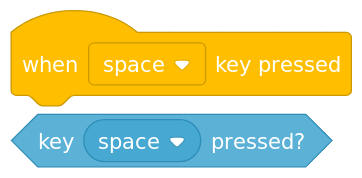
\includegraphics[scale=1.5]{scratch-input-blocks-1}\vspace{2mm} & \tablebox{$\rightarrow$ Press the respective keyboard key}                \\
        \vspace{3.5mm}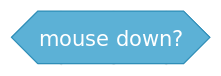
\includegraphics[scale=1.5]{scratch-input-blocks-2}\vspace{2mm} & \tablebox{$\rightarrow$ Click the left mouse button}                      \\
        \vspace{3.5mm}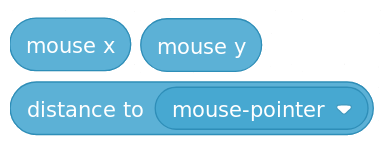
\includegraphics[scale=1.5]{scratch-input-blocks-3}\vspace{2mm} & \tablebox{$\rightarrow$ Move the cursor to a random position}             \\
        \vspace{3.5mm}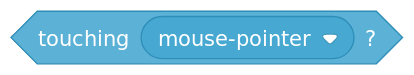
\includegraphics[scale=1.5]{scratch-input-blocks-4}\vspace{2mm} & \tablebox{$\rightarrow$ Move the cursor near / onto the respective sprite \\
                                                                                                  $\rightarrow$ Move the cursor to a random position}             \\
        \vspace{3.5mm}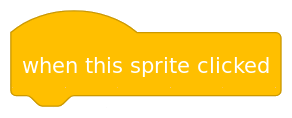
\includegraphics[scale=1.5]{scratch-input-blocks-5}\vspace{2mm} & \tablebox{$\rightarrow$ Click near / onto the respective sprite           \\
                                                                                                  $\rightarrow$ Click on a random position}                       \\
        \vspace{3.5mm}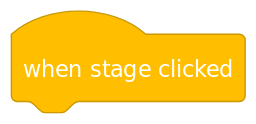
\includegraphics[scale=1.5]{scratch-input-blocks-6}\vspace{2mm} & \tablebox{$\rightarrow$ Click on a random position}                       \\
        \vspace{3.5mm}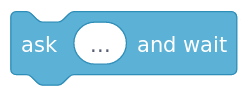
\includegraphics[scale=1.5]{scratch-input-blocks-7}\vspace{2mm} & \tablebox{$\rightarrow$ Answer with a randomly generated string}          \\
        \vspace{3.5mm}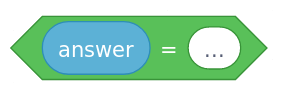
\includegraphics[scale=1.5]{scratch-input-blocks-8}\vspace{2mm} & \tablebox{$\rightarrow$ Answer with the compared string constant}         \\
        \bottomrule
    \end{tabular}

    \caption{Scratch's input blocks and their resulting generated inputs}
    \label{tab:scratch_input_blocks}

    \renewcommand{\baselinestretch}{\oldbls}
\end{table}

\section{Callbacks and Constraints}

Callbacks and constraints are both JavaScript functions,
which are registered to be called periodically during the program execution.
When they are registered, they are simply put into a list.
Then, during the step procedure,
Whisker iterates over both lists and executes every callback and constraint.
Both callbacks and constraints can be enabled and disabled,
which adds or removes them from their respective list.
\parspace

Constraints have on key difference to normal callbacks:
They catch assertion errors.
Whenever an assertion error is caught while executing a constraint,
the constraint is removed from the list,
and the error is forwarded to the VM wrapper.
This makes it possible to react to failed constraints in different ways.
The VM wrapper can, depending on configuration, re-throw the error to fail the test,
stop the current run of the program,
or ignore the constraint failure entirely.

\section{Coverage Measurement}

Whisker can be used to measure statement coverage on a Scratch program.
It does this by temporarily modifying Scratch's \texttt{Thread} class.
This class has two methods, \texttt{pushStack} and \texttt{reuseStackForNextBlock},
which push blocks on top of the execution stack.
Whisker intercepts these methods by replacing them with a version,
which saves the unique id of the executed blocks and then calls the respective original method.
This way, Whisker can track which blocks are executed by the program.
\parspace

In order to calculate the coverage, Whisker also needs a list of the program's blocks.
To compose this list, Whisker traverses all scripts of the program currently loaded by the virtual machine,
and saves each block's unique id.
Because Whisker traverses the scripts, blocks, which are not part of a script with a hat,
are ignored for the coverage measurement.
This is not a problem, because these blocks will never be covered anyways,
since they are not reachable by the program.
\parspace

Coverage is measured per sprite, but program wide coverage can also be calculated.
Listing~\ref{fig:example_coverage_report} shows an example coverage report.
Listing~\ref{fig:measuring_coverage} gives a code example of how to measure statement coverage with Whisker.
\parspace

\begin{listing}[htpb]
    \centering

    \begin{minipage}{.5\textwidth}
        \begin{javascriptcode}
            {
                stage: { covered: 0, total: 0 },
                bowl: { covered: 16, total: 16 },
                bananas: { covered: 12, total: 24 },
                apple: { covered: 15, total: 18 }
            }
        \end{javascriptcode}
    \end{minipage}

    \caption{Example coverage report}
    \label{fig:example_coverage_report}
\end{listing}

% \begin{enumerate}[(1)]
%     \item \texttt{prepareThread} replaces methods in \texttt{Thread}, so coverage can be tracked.
%     \item \texttt{prepare} traverses the program and gathers a list of all reachable blocks.
%     \item \texttt{getCoverage} calculates the coverage and returns it.
%     \item \texttt{restoreThread} restores \texttt{Thread}'s original method implementations.
% \end{enumerate}

% \begin{enumerate}[(1)]
%     \item \texttt{prepareThread} replaces the \texttt{pushStack} and \texttt{reuseStackForNextBlock} methods of the \texttt{Thread} class.
%         The new methods simply track the block, which is put on the execution stack, and then call the respective original method.
%     \item \texttt{prepare} traverses the scripts of the program, which is currently loaded by the virtual machine, and gathers a list of the program's blocks.
%         Whisker only gathers reachable blocks, i.e. blocks, which are part of a script equipped with a hat.
%         Therefore, unreachable blocks are ignored for the coverage measurement.
%     \item \texttt{getCoverage} calculates the coverage based on the program's blocks and the blocks, which are known to be used by a thread.
%     \item \texttt{restoreThread} restores the original method implementations of the \texttt{Thread} class.
% \end{enumerate}

\begin{listing}[htpb]
    \centering

    \begin{minipage}{.75\textwidth}
        \begin{javascriptcode}
            /* (1) Replace pushStack and reuseStackForNextBlock,
               so the executed blocks can be tracked. */
            CoverageGenerator.prepareThread(Thread);

            /* (2) Traverse the scripts of the currently loaded program
               and gather a list of all reachable blocks. */
            CoverageGenerator.prepare(vm);

            /* Run the Scratch program. */
            ...

            /* (3) Retrieve the current statement coverage. */
            const coverage = CoverageGenerator.getCoverage();

            /* (4) Restore real implementations of pushStack and
               reuseStackForNextBlock. */
            CoverageGenerator.restoreThread(Thread);
        \end{javascriptcode}
    \end{minipage}

    \caption{Example of how to measure coverage using Whisker}
    \label{fig:measuring_coverage}
\end{listing}

In order to measure coverage, one has to gain access to Scratch's \texttt{Thread} class.
This can be achieved either at compile time or at runtime.
Listing~\ref{fig:acquiring_thread_class} shows example code of how this can be done.
\parspace

\begin{listing}[htpb]
    \centering

    \begin{subfigure}[b]{.7\textwidth}
        \begin{javascriptcode}
            const VirtualMachine = require('scratch-vm');
            const Thread = require('scratch-vm/src/engine/thread');
        \end{javascriptcode}
        \vspace{-\bigskipamount}
        \caption{At compile time using JavaScript's module system}
    \end{subfigure}

    \bigskip

    \begin{subfigure}[b]{.7\textwidth}
        \begin{javascriptcode}
            const Thread = vm.runtime.threads[0].__proto__
        \end{javascriptcode}
        \vspace{-\bigskipamount}
        \caption{At runtime by getting the class of a running \texttt{Thread} instance}
    \end{subfigure}

    \caption{Examples of how to acquire Scratch's \texttt{Thread} class}
    \label{fig:acquiring_thread_class}
\end{listing}

% \section{Running Tests}
%
% Since Whisker itself is just an automation tool,
% it can theoretically be used with any JavaScript testing framework.
%
% - Whisker comes with an optional testing framework
% - Include a sample test report?
%
% === Seeing test output, interactive tests
% - Users will want to see the program's output while it is run
%     - to check if the tests run correctly, to check if the program runs correctly
%     - Difficult to determine a problem with the project from just textual test reports
%     - Tests without showing output are not very useful in such an interactive environment
% $\rightarrow$ Has to be able to run in a interactive environment
%     - Web GUI, which can be run by any modern browser
%     - Allows users to run individual tests on the project and see the program execution
%
% === Batch Testing of Projects
% - Some tests for Scratch projects can take a long time because projects run in real time
%     - raises the need to test scratch programs in parallel
%     - Scratch depends on the renderer
%         - Some functionality of the Scratch virtual machine depends on the renderer
%         - Headless tests are impossible without restricting the Scratch program to a subset of available blocks
% $\rightarrow$ Web GUI has the option to run tests on multiple projects sequentially, but this might still take a long time depending on the project and the test suite
% $\rightarrow$ Electron
%     - Running tests in multiple processes could circumvent the problem
%     - Electron provides a renderer that can be used to render the Scratch output to
%     - Spawns multiple processes which open a window each, one project is tested in each window

% \section{Basic Testing Functionality}
%
% === WM Wrapper
% - Control the execution of the scratch program
% - Run the program until a certain amount of time has passed or a condition has been met
% - Get the time elapsed since the start of the test or the start of the last run
% - Cancel a run
% - Uses JavaScript's Promise API to wait until a run is finished
%
% \begin{listing}[htpb]
%     \centering
%     \begin{javascriptcode}
%         await t.runForTime(500);
%         await t.runUntil(() => !t.projectRunning(), 1000);
%         t.assert.ok(t.getTotalTimeElapsed() < 1000);
%     \end{javascriptcode}
%     \vspace{-\bigskipamount}
%     \caption{Example code for the VM Wrapper}
%     \label{fig:example_code_for_the_vm_wrapper}
% \end{listing}
%
% === Sprites
% - Sprite is not the same as sprite in Scratch VM
%     - Explain distinguishes between sprites and targets / rendered targets
%     - Sprite contains the blocks, graphics (costumes), etc.
%     - Target / rendered target is an instance of the sprite
%     - Whisker sees every rendered target as a sprite
%     - The original target of a Scratch sprite as well as its clones are each an instance of a ''sprites''
%     - TODO: explain clones here
%
% - Sprites work by wrapping around the original
% - If some getter of the sprite is called, the actual value is retrieved from the original target
% - Most properties are implemented as JavaScript getters $\rightarrow$ look like properties of Whisker's sprite object
%
% - Information about sprites and variables
% - Gives the information that the test uses
% - Does not allow to manipulate sprites and variables
% - Contains ''old'' value for every fitting property
%     - Saves the value from the last step
%     - Useful for constraints (see later)
%     - Initialized with the present value
% - Sprites are only tracked once they are retrieved via one of the getter method
% - Helps, for example, with programs that spawn a lot of clones (could pose a performance problem otherwise)
%
%
% \begin{listing}[htpb]
%     \centering
%     \begin{javascriptcode}
%         const sprite = t.getSprite('Sprite1');
%         const variable = sprite.getVariable('Variable1');
%         const sprites = t.getSprites(s => s.x > 100);
%
%         t.assert.equal(sprite.x, 100);
%         t.assert.equal(sprite.old.x, 100);
%         t.assert.equal(variable.value, 5);
%     \end{javascriptcode}
%     \vspace{-\bigskipamount}
%     \caption{Example code for Sprites}
%     \label{fig:example_code_for_sprites}
% \end{listing}
%
% === Inputs
% - INPUTS ARE SIMULATED ON THE VM, NO ACTIONS ARE SIMULATED ON THE OS LEVEL OR ANYTHING
%
% - Simulate inputs on the program
% - Can be registered to be called after a certain amount of time or be executed immediately
% - Registering a Input with 0 delay is different from executing it immediately
% === Kinds of Input
% - At the moment: only mouse and keyboard input
% - Keyboard:
%     - Press a key
%     - Release a key
%     - Toggle a key
%     - Press / release a key for a certain duration
% - Mouse (only left mouse button):
%     - move cursor to position
%     - move cursor to sprite (+offset)
%     - press mouse button
%     - release mouse button
%     - toggle mouse button
%     - Press / release mouse button for a certain duration
%
% \begin{listing}[htpb]
%     \centering
%     \begin{javascriptcode}
%         t.inputImmediate({
%             device: 'keyboard',
%             key: 'right arrow',
%             isDown: true
%         });
%
%         const mouseInput = t.addInput(1000, {
%             device: 'mouse',
%             x: 100,
%             y: 0,
%             isDown: true,
%             duration: 500
%         });
%
%         t.assert.ok(t.isKeyDown('right arrow'));
%         t.removeInput(mouseInput);
%         t.addInput(mouseInput);
%     \end{javascriptcode}
%     \vspace{-\bigskipamount}
%     \caption{Example code for Random Inputs}
%     \label{fig:example_code_for_random_inputs}
% \end{listing}
%
% === Random Inputs
% - Provides a simple way to perform inputs randomly
% - Way of testing the program without deliberately controlling the inputs
% - In a set time interval (at the next step), an input is randomly selected from a pool of registered random inputs
%
% - You  can register inputs for the random pool, or let Whisker choose inputs based on the blocks used in the program
% - Random inputs can be detected through simple static analysis
% $\rightarrow$ Blocks that take inputs and their options are analyzed
%
% - TODO table of detected blocks and resulting inputs ?
%
% \begin{listing}[htpb]
%     \centering
%     \begin{javascriptcode}
%         t.setRandomInputInterval(150);
%         t.registerRandomInputs([
%             {
%                 device: 'keyboard',
%                 key: 'left arrow',
%                 duration: [50, 100]
%             },
%             {
%                 device: 'keyboard',
%                 key: 'right arrow',
%                 duration: [50, 100]
%             }
%         ]);
%         t.detectRandomInputs();
%     \end{javascriptcode}
%     \vspace{-\bigskipamount}
%     \caption{Example code for Inputs}
%     \label{fig:example_code_for_inputs}
% \end{listing}
%
% === Callbacks
% - Register callbacks that are called after every step
% - Can be registered to run at two positions in the step cycle (see diagram later)
% - Purpose:
%     - Information Tracking:
%         - Track events
%         - e.g how many times a sprite touches some other sprite
%               or how long a sprite is invisible, etc.
%     - Inputs:
%         - Allows performing conditional inputs
%         - Control the program like a player would
%         - e.g. follow a sprite with the mouse cursor
%
% \begin{listing}[htpb]
%     \centering
%     \begin{javascriptcode}
%         const sprite = t.getSprite('Sprite1');
%
%         const callback = t.addCallback(() => {
%             t.inputImmediate({
%                 device: 'mouse',
%                 x: sprite.x,
%                 y: sprite.y
%             });
%         });
%
%         await t.runForTime(1000);
%
%         callback.disable();
%         callback.enable();
%     \end{javascriptcode}
%     \vspace{-\bigskipamount}
%     \caption{Example code for Callbacks}
%     \label{fig:example_code_for_callbacks}
% \end{listing}
%
%
% === Constraints
% - Describe conditions that must always hold
% - Failed constraints can be configured to fail the test, stop the current program run (\texttt{run...()}), or do nothing
% - Can be used to perform checks like "sprite xy is always visible when sprite yz is visible"
% - Implemented as callbacks that execute assertions
%     - Advantages:
%         - Concise syntax
%         - Multiple assertions per constraint possible
%         - Assertion messages can be used to describe the constraint failure
%     - Disadvantages:
%         - Assertion methods have to be efficient, e.g. if assertion message is constructed every time it could be too slow
%         - Need to catch exceptions if constraints should not fail the test
% - Can separate assertions from the program execution
%     - Define constraints for tested properties, then use whatever input (deliberate / random / manual)
%     - Problem: most constraints still hold if the tested property is not implemented at all
%         - e.g. constraint that checks that a sprite never moves left will hold if the sprite doesn't move at all
%
% \begin{listing}[htpb]
%     \centering
%     \begin{javascriptcode}
%         const sprite = t.getSprite('Sprite1');
%
%         t.onConstraintFailure('fail');
%
%         const constraint = t.addConstraint(() => {
%             t.assert.ok(sprite.x >= sprite.old.x);
%         });
%
%         await t.runForTime(1000);
%
%         constraint.disable();
%     \end{javascriptcode}
%     \vspace{-\bigskipamount}
%     \caption{Example code for Constraints}
%     \label{fig:example_code_for_constraints}
% \end{listing}
